%%%%%%%%%%%%%%%%%%%%%%%%%%%%%%%%%%%%%%%%%%%%%%%%%%%%%%%%%%%%%%%%%%%%%%%%
%    INSTITUTE OF PHYSICS PUBLISHING                                   %
%                                                                      %
%   `Preparing an article for publication in an Institute of Physics   %
%    Publishing journal using LaTeX'                                   %
%                                                                      %
%    LaTeX source code `ioplau2e.tex' used to generate `author         %
%    guidelines', the documentation explaining and demonstrating use   %
%    of the Institute of Physics Publishing LaTeX preprint files       %
%    `iopart.cls, iopart12.clo and iopart10.clo'.                      %
%                                                                      %
%    `ioplau2e.tex' itself uses LaTeX with `iopart.cls'                %
%                                                                      %
%%%%%%%%%%%%%%%%%%%%%%%%%%%%%%%%%%
% 
% git: git push all master	
%
% First we have a character check
%
% ! exclamation mark    " double quote  
% # hash                ` opening quote (grave)
% & ampersand           ' closing quote (acute)
% $ dollar              % percent       got
% ( open parenthesis    ) close paren.  
% - hyphen              = equals sign
  
  % 23 
  
  % 23 
% | vertical bar        ~ tilde         
% @ at sign             _ underscore
% { open curly brace    } close curly   
% [ open square         ] close square bracket
% + plus sign           ; semi-colon    
% * asterisk            : colon
% < open angle bracket  > close angle   
% , comma               . full stop
% ? question mark       / forward slash 
% \ backslash           ^ circumflex
%
% ABCDEFGHIJKLMNOPQRSTUVWXYZ 
% abcdefghijklmnopqrstuvwxyz 
% 1234567890
%
%%%%%%%%%%%%%%%%%%%%%%%%%%%%%%%%%%%%%%%%%%%%%%%%%%%%%%%%%%%%%%%%%%%
%
\pdfminorversion=4
\documentclass[12pt]{iopart}
\newcommand{\gguide}{{\it Preparing graphics for IOP Publishing journals}}
%Uncomment next line if AMS fonts required
\usepackage{iopams}  
\usepackage{tabularx}
\usepackage{multirow}
\usepackage{graphicx}
\usepackage{color}
\usepackage[english]{babel}
% \usepackage{harvard}  
\usepackage{natbib}
\usepackage{lineno}
\linenumbers*[1]

\begin{document}
	
\title[Silage Maize Yield Estimates using Soil Moisture Climate Projections]{Silage Maize Yield estimates using Soil Moisture Climate Projections}
\author{Michael Peichl$^1$, Stephan Thober$^1$, Luis Samaniego$^1$, Bernd Hansjuergens$^1$, Andreas Marx$^{1,2}$}

\address{$^1$ Department Computational Hydrosystems, Helmholtz Centre for Environmental Research - UFZ, Permoserstrasse 15, D-04318 Leipzig, Germany}
\address{$^2$ Climate Office for Central Germany, Helmholtz Centre for Environmental Research - UFZ, Permoserstrasse 15, D-04318 Leipzig, Germany}
\ead{michael.peichl@ufz.de}

\begin{abstract}
Silage maize is one of the most widespread cultivated plants in Germany because it is a main supplier of biomass in the course of the energy transition. Silage maize yield is susceptible to unfavorable environmental conditions such as dry and wet spells. Knowledge of these factors can help to mitigate welfare losses and can be used to estimate the impact of climate change on crop yields. 
Statistical crop models routinely use meteorological variations to estimate crop yield although soil moisture constitutes the primary source of water for plant growth. In an earlier study, the intra-seasonal predictive capacity of soil moisture for the estimation of silage maize yields in Germany was investigated  (Peichl et al. 2018). The main result is that soil moisture anomalies have exploratory skills which vary in magnitude and direction depending on the month. 
The most important seasonal effects are then combined here in a reduced panel model to enable a more holistic climate impact assessment. These effects are soil moisture of June and August, which show opposite detrimental effects, and July temperature and precipitation. It is worth noting that the models used in this study neglect effects such as increased CO$_2$ fertilization and agricultural adaptation measures.  
To estimate soil  moisture anomalies, climate projections derived from five regional climate models (RCMs) of the ENSEMBLES project under A1B scenario are used to force the mesoscale Hydrological Model (www.ufz.de/mHM). The meteorological data are demeaned to correct for systematic biases of the RCMs. The approach is based solely on anomalies. Silage maize yield variations are predicted for the reference period 1971 – 2000 and projected for the climate periods  2021 - 2050 and 2070 - 2099. For all RCMs, on average crop yield is projected to decrease for both climate periods ranging from -1.2 to -10.5 decitonnes/hectar (dt/ha) for the period 2021 – 2050 and -3.7 to -39.1 dt/ha until the end of the century. The maximum projected yield loss is less than 10 \% of the average yield in Germany for the period 1999 – 2015 (447  dt/ha). Among the different explanatory variables no single driver of crop yield anomalies could be identified. This highlights that multiple seasonal determinants are required for accurate estimation of crop yield variation. 


% 

\end{abstract}

\noindent{\it Keywords\/}: silage maize, climate change, Germany (3 - 7 words)

%\keywords{magnetic moment, solar neutrinos, astrophysics}

%Uncomment for PACS numbers title message
%\pacs{00.00, 20.00, 42.10}
% Keywords required only for MST, PB, PMB, PM, JOA, JOB? 
%\vspace{2pc}
%\noindent{\it Keywords}: Article preparation, IOP journals
% Uncomment for Submitted to journal title message
\submitto{\ERL}
% Comment out if separate title page not required
\maketitle


\section{Introduction}
Based on the current research on silage maize sensitivity to monthly weather and soil moisture impacts  a predictive model shall be established.  So far, the goal was to evaluate the causal effects of soil moisture anomalies on a monthly basis. So far, time dependent effects of soil moisture have been evaluated. For instance extreme wetness in the early period and extreme dryness in August are responsible for diminished silage maize yield.  Further, the focus was on in-sample variation. This has methodological implications, as for instance the use of parametric standard errors and the control for confounding factors. Also, it allows to use plm package, which is not so good suited for predictions. 
Now, we derive heuristacially a model which relies on the seasonal effects observed in the paper before. 

Literature:
IPCC: AR5 (Synthesis Report)
Distribution of Impacts (Figure SPM.10)

For the major crops (wheat, rice, and maize) in tropical and temperate regions, climate change without adaptation is projected to negatively impact production for local temperature increases of 2°C or more above late-20th- century levels, although individual locations may benefit (medium confidence).



\section{Data and Methods}
\subsection{Training Data}

\label{data:1}
% Fig 1 
% include graphics
\begin{figure}
	\label{f:1}
	\centering
	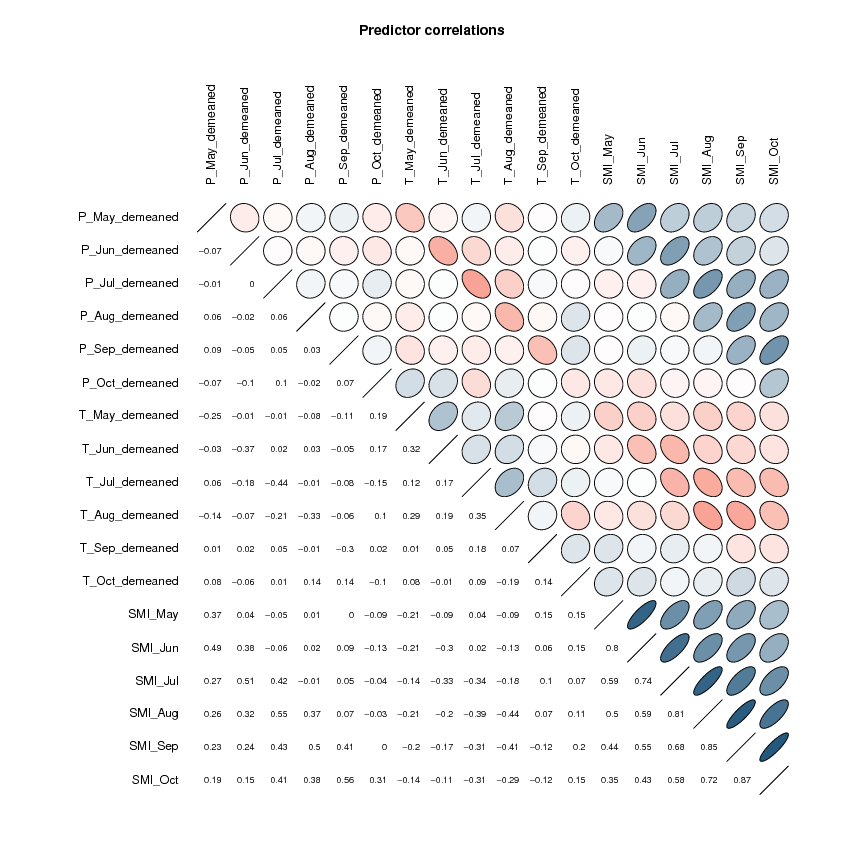
\includegraphics[width=1\textwidth]{figures/PredictorCorrelation.png}
	\caption{Pearson Correlation of the possible predictors used in the model.}
\end{figure}

% Table created by stargazer v.5.2 by Marek Hlavac, Harvard University. E-mail: hlavac at fas.harvard.edu
% Date and time: Mi, Jan 03, 2018 - 12:26:52
\begin{table}[!htbp] \centering 
	\caption{} 
	\label{} 
	{\tiny
	\begin{tabular}{@{\extracolsep{5pt}}lcc} 
		\\[-1.8ex]\hline 
		\hline \\[-1.8ex] 
		& \multicolumn{2}{c}{Base Model} \\ 
		\cline{2-3} 
		\\[-1.8ex] & \multicolumn{2}{c}{silomaize} \\ 
		& Standard & Driscol - Kraay \\ 
		\hline \\[-1.8ex] 
		poly(P\_Jul)$^{1}$ & 0.264$^{***}$ & 0.264$^{***}$ \\ 
		& (0.028) & (0.033) \\ 
		& & \\ 
		poly(P\_Jul)$^{2}$ & 0.001$^{**}$ & 0.001 \\ 
		& (0.0003) & (0.001) \\ 
		& & \\ 
		poly(P\_Jul)$^{3}$ & $-$0.00001$^{***}$ & $-$0.00001$^{**}$ \\ 
		& (0.00000) & (0.00000) \\ 
		& & \\ 
		poly(T\_Jul)$^{1}$ & $-$6.443$^{***}$ & $-$6.443$^{***}$ \\ 
		& (0.634) & (1.001) \\ 
		& & \\ 
		poly(T\_Jul)$^{2}$ & $-$4.050$^{***}$ & $-$4.050$^{***}$ \\ 
		& (0.305) & (0.291) \\ 
		& & \\ 
		poly(T\_Jul)$^{3}$ & 0.703$^{***}$ & 0.703$^{***}$ \\ 
		& (0.078) & (0.104) \\ 
		& & \\ 
		SMI\_Jun6drght\_svr & 10.622$^{***}$ & 10.622$^{***}$ \\ 
		& (2.196) & (2.880) \\ 
		& & \\ 
		SMI\_Jun6drght\_mdrt & 8.723$^{***}$ & 8.723$^{***}$ \\ 
		& (1.988) & (2.303) \\ 
		& & \\ 
		SMI\_Jun6dry & 3.198$^{*}$ & 3.198$^{*}$ \\ 
		& (1.722) & (1.763) \\ 
		& & \\ 
		SMI\_Jun6wt & $-$6.155$^{***}$ & $-$6.155$^{**}$ \\ 
		& (2.203) & (2.462) \\ 
		& & \\ 
		SMI\_Jun6wt\_abndnt & $-$12.173$^{***}$ & $-$12.173$^{***}$ \\ 
		& (2.660) & (3.813) \\ 
		& & \\ 
		SMI\_Jun6wt\_svr & $-$52.091$^{***}$ & $-$52.091$^{***}$ \\ 
		& (3.618) & (5.850) \\ 
		& & \\ 
		SMI\_Aug6drght\_svr & $-$47.447$^{***}$ & $-$47.447$^{***}$ \\ 
		& (2.609) & (3.820) \\ 
		& & \\ 
		SMI\_Aug6drght\_mdrt & $-$21.952$^{***}$ & $-$21.952$^{***}$ \\ 
		& (2.066) & (2.837) \\ 
		& & \\ 
		SMI\_Aug6dry & $-$8.200$^{***}$ & $-$8.200$^{***}$ \\ 
		& (1.771) & (2.495) \\ 
		& & \\ 
		SMI\_Aug6wt & 0.656 & 0.656 \\ 
		& (2.084) & (1.800) \\ 
		& & \\ 
		SMI\_Aug6wt\_abndnt & $-$3.447 & $-$3.447 \\ 
		& (2.428) & (2.431) \\ 
		& & \\ 
		SMI\_Aug6wt\_svr & $-$10.703$^{***}$ & $-$10.703$^{***}$ \\ 
		& (3.548) & (3.755) \\ 
		& & \\ 
		Constant & 18.905$^{***}$ & 18.905$^{***}$ \\ 
		& (1.155) & (1.527) \\ 
		& & \\ 
		\hline \\[-1.8ex] 
		Observations & 4,625 & 4,625 \\ 
		R$^{2}$ & 0.389 & 0.389 \\ 
		Adjusted R$^{2}$ & 0.387 & 0.387 \\ 
		F Statistic (df = 18; 4606) & 162.900$^{***}$ & 162.900$^{***}$ \\ 
		\hline 
		\hline \\[-1.8ex] 
		\textit{Note:}  & \multicolumn{2}{r}{$^{*}$p$<$0.1; $^{**}$p$<$0.05; $^{***}$p$<$0.01} \\ 
	\end{tabular} 
	 }
\end{table} 

\begin{itemize}
\item Here I should 
\end{itemize}



\subsection{Method}
\subsubsection{Model without fixed effects but demeaned data.}
Combined model from paper 1, excluding the fixed effects. Here, test for fixed effects can be included. In that context we also can mention some interpretation particularities (together with using anomalies in the predictor variables.)

\subsubsection{Test Results}

\subsection{Climate Data}
\begin{figure}
	\label{climateData:1f}
	\centering
	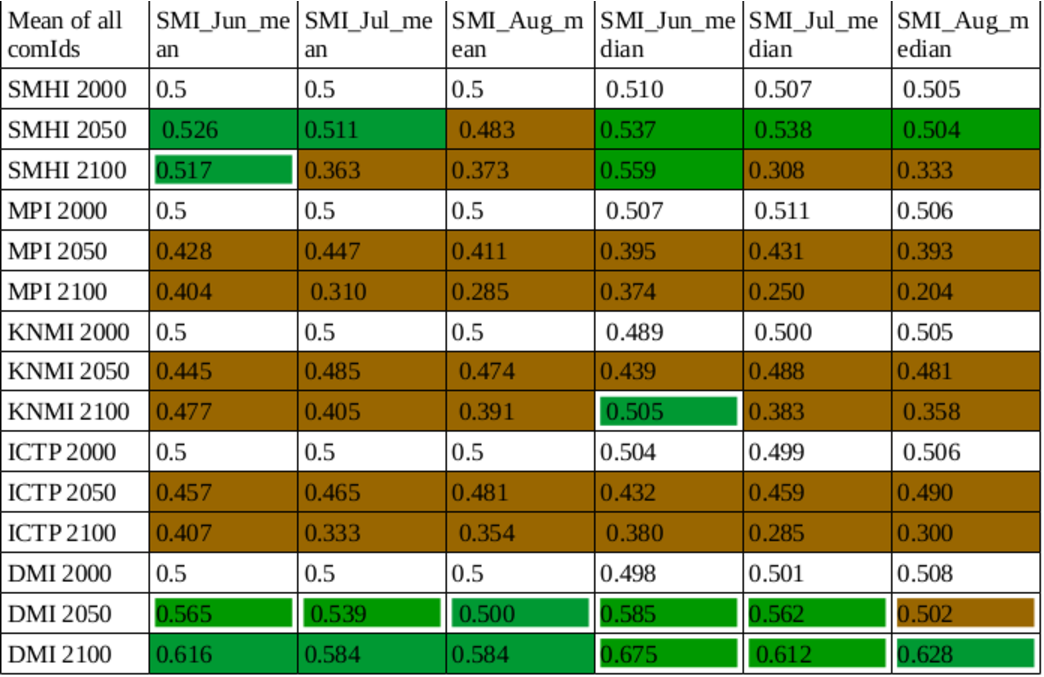
\includegraphics[width=1\textwidth]{figures/MeanofSMI.pdf}
	\caption{Comparision of the SMI develpment of each RCM.}
\end{figure}

\section{Results and Discussion}
\subsection{Goodness of Fit and Model Coefficients}
In and out of sample goodness of fit.

\subsection{Scatter-plot}

\label{scatter:1}

\begin{figure}
	\label{scatter:1f}
	\centering
	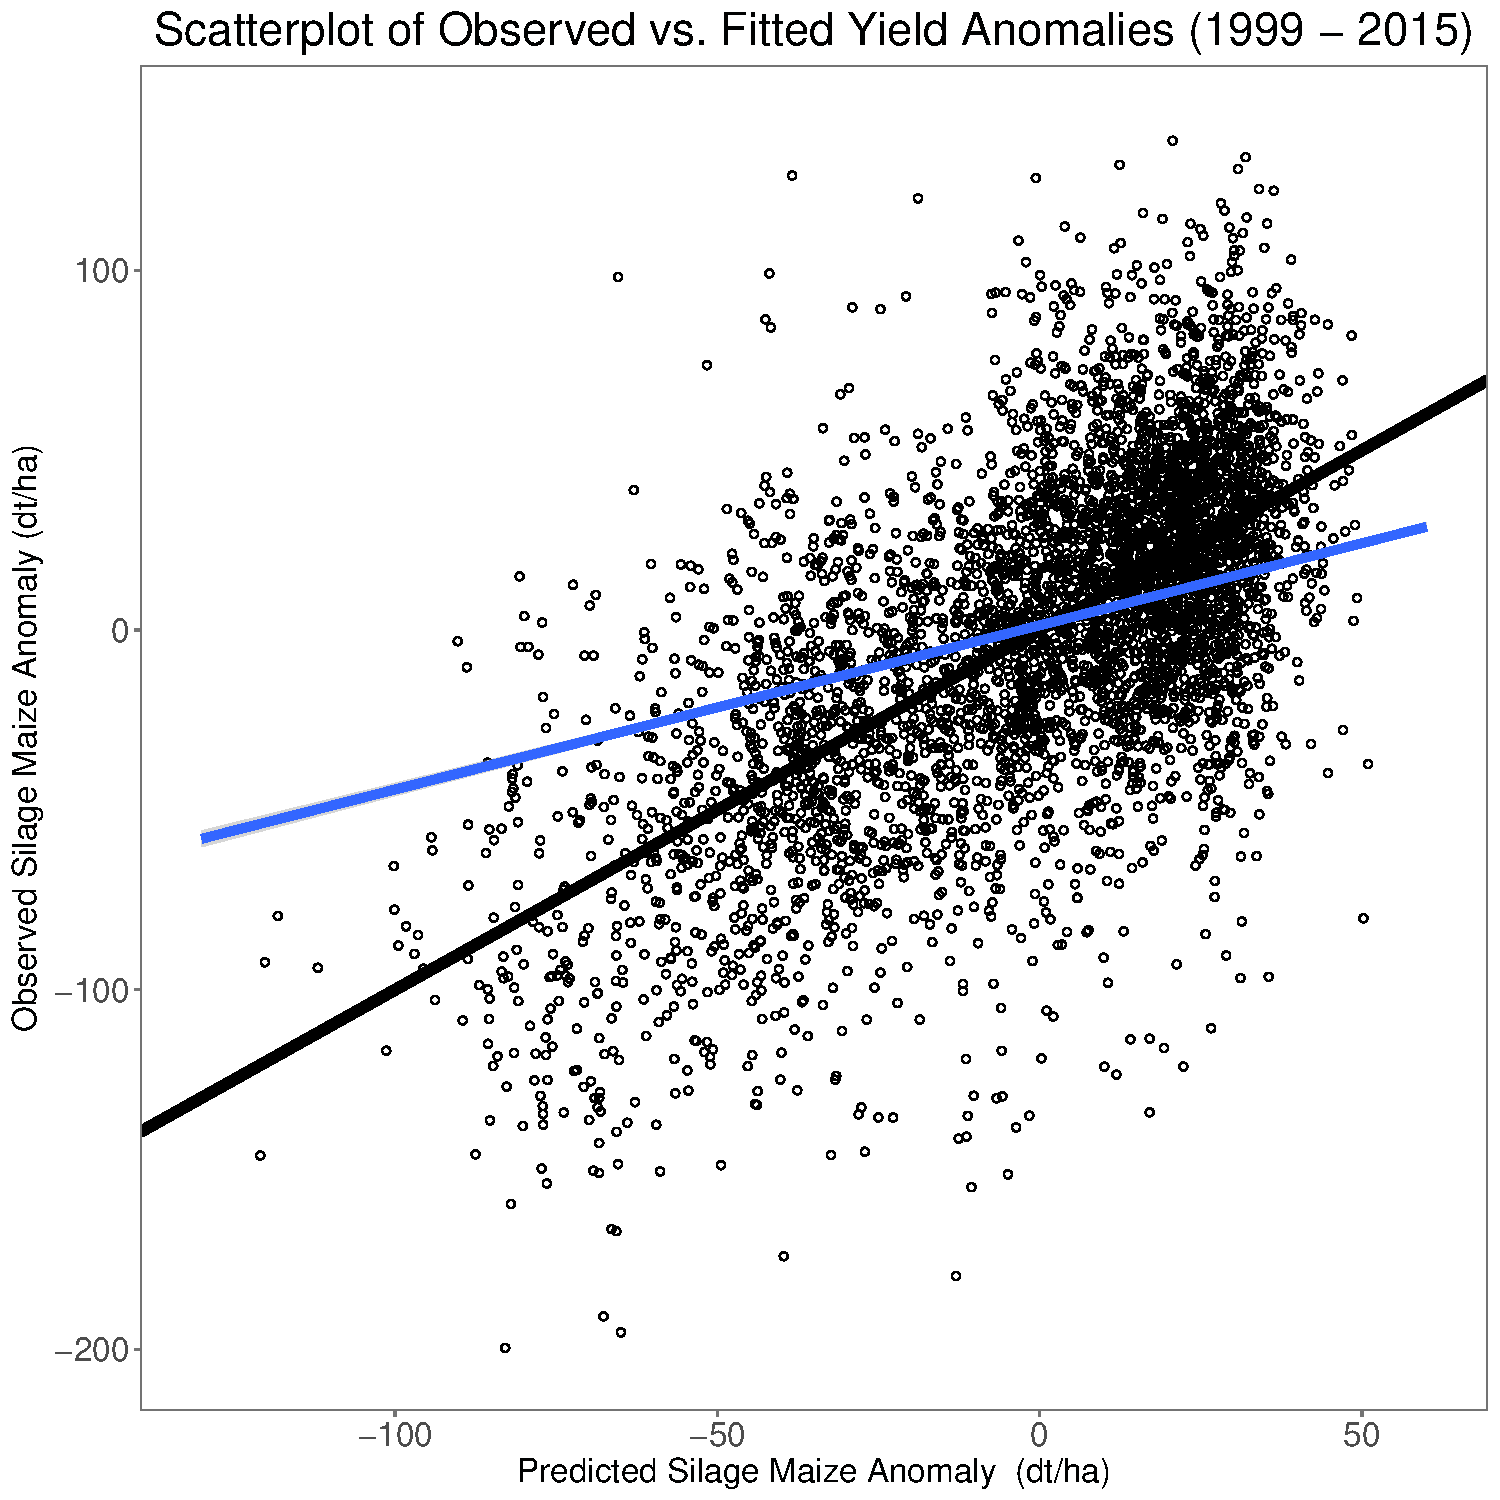
\includegraphics[width=1\textwidth]{figures/Train_1999-2015.pdf}
	\caption{Scatterplot of the observed silage Maize Anomaly Data against the predicted data. The time period is 1999 to 2015.}
\end{figure}

\begin{figure}
	\label{scatter:2f}
	\centering
	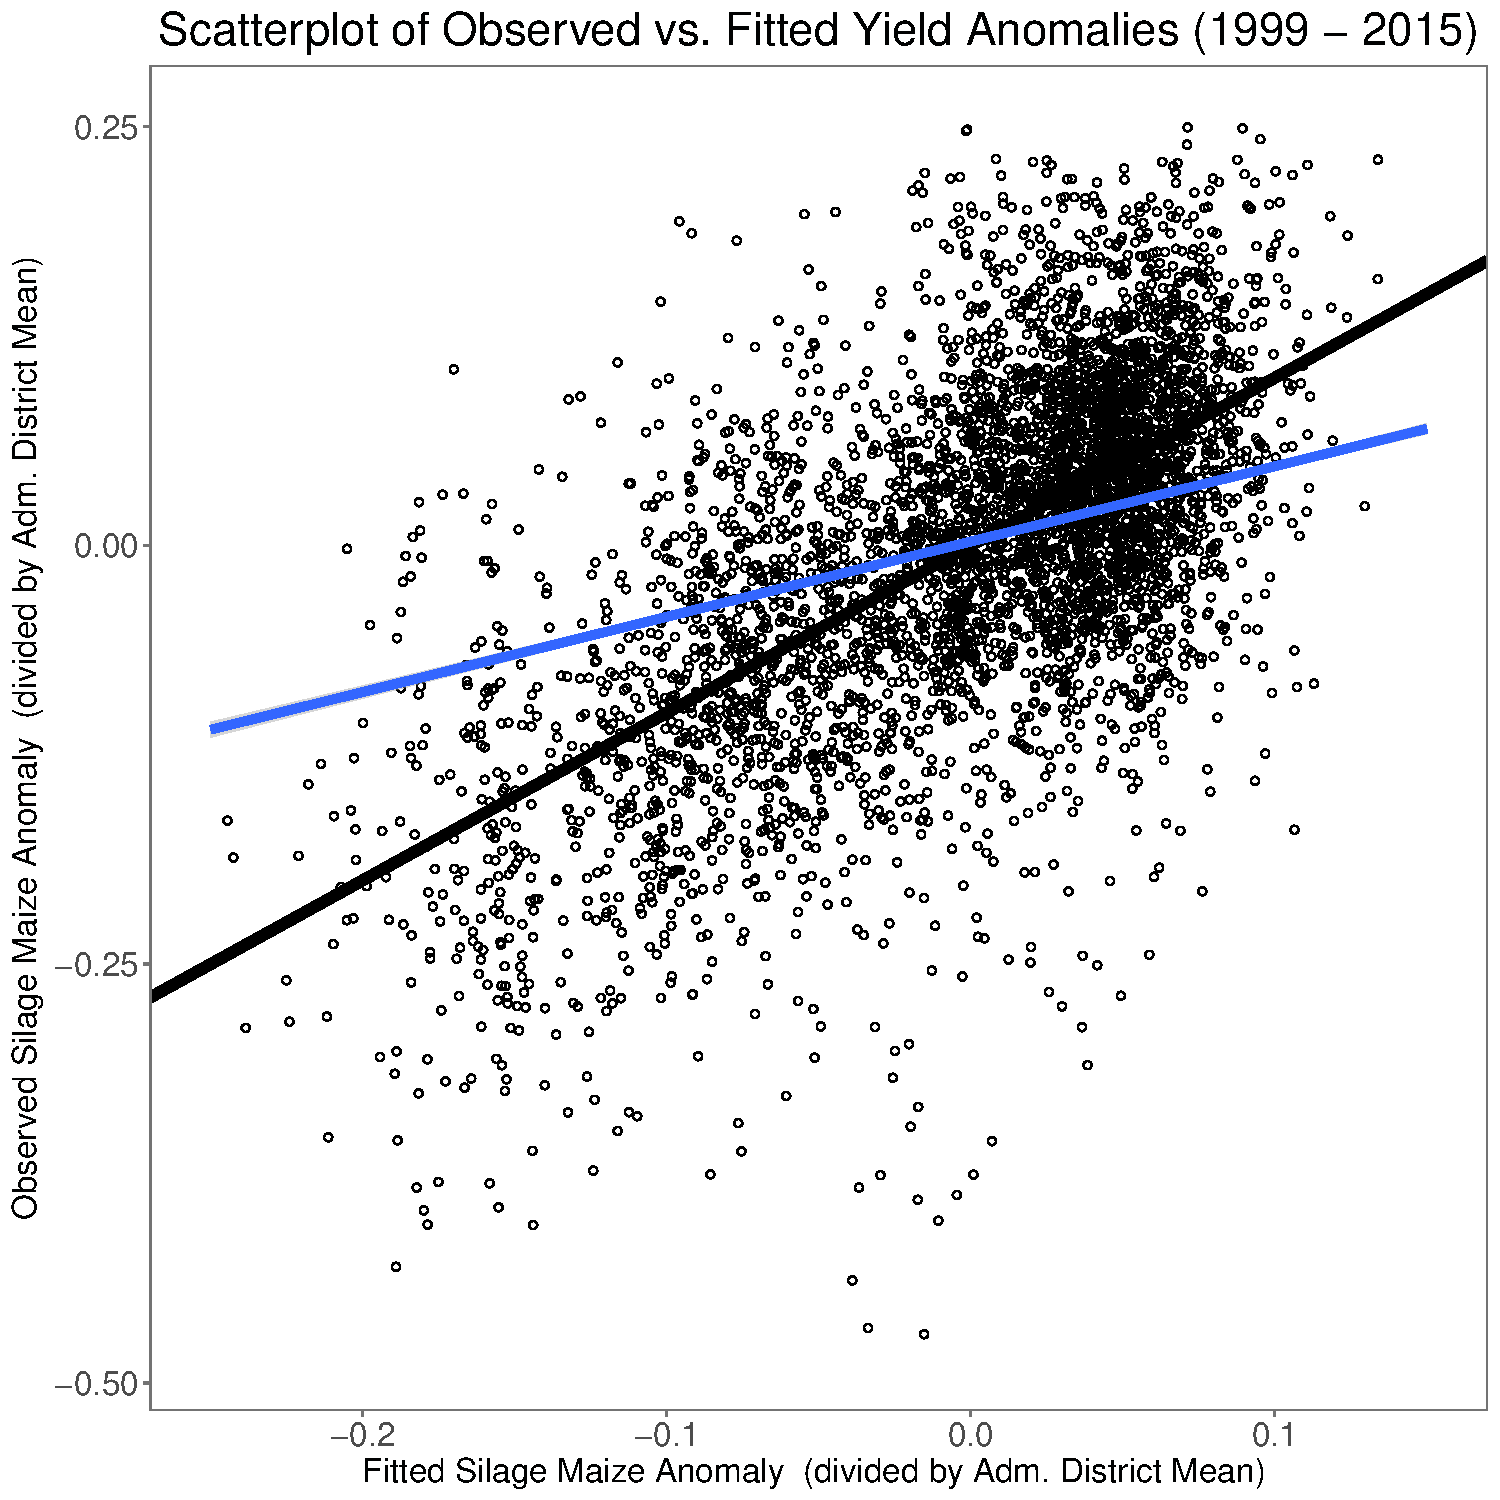
\includegraphics[width=1\textwidth]{figures/Train_1999-2015_norm.pdf}
	\caption{Scatterplot of the observed silage Maize Anomaly Data against the predicted data (both divided by the observed mean yield of each administrative district). The time period is 1999 to 2015.}
\end{figure}


\begin{figure}
	\label{density:1f}
	\centering
	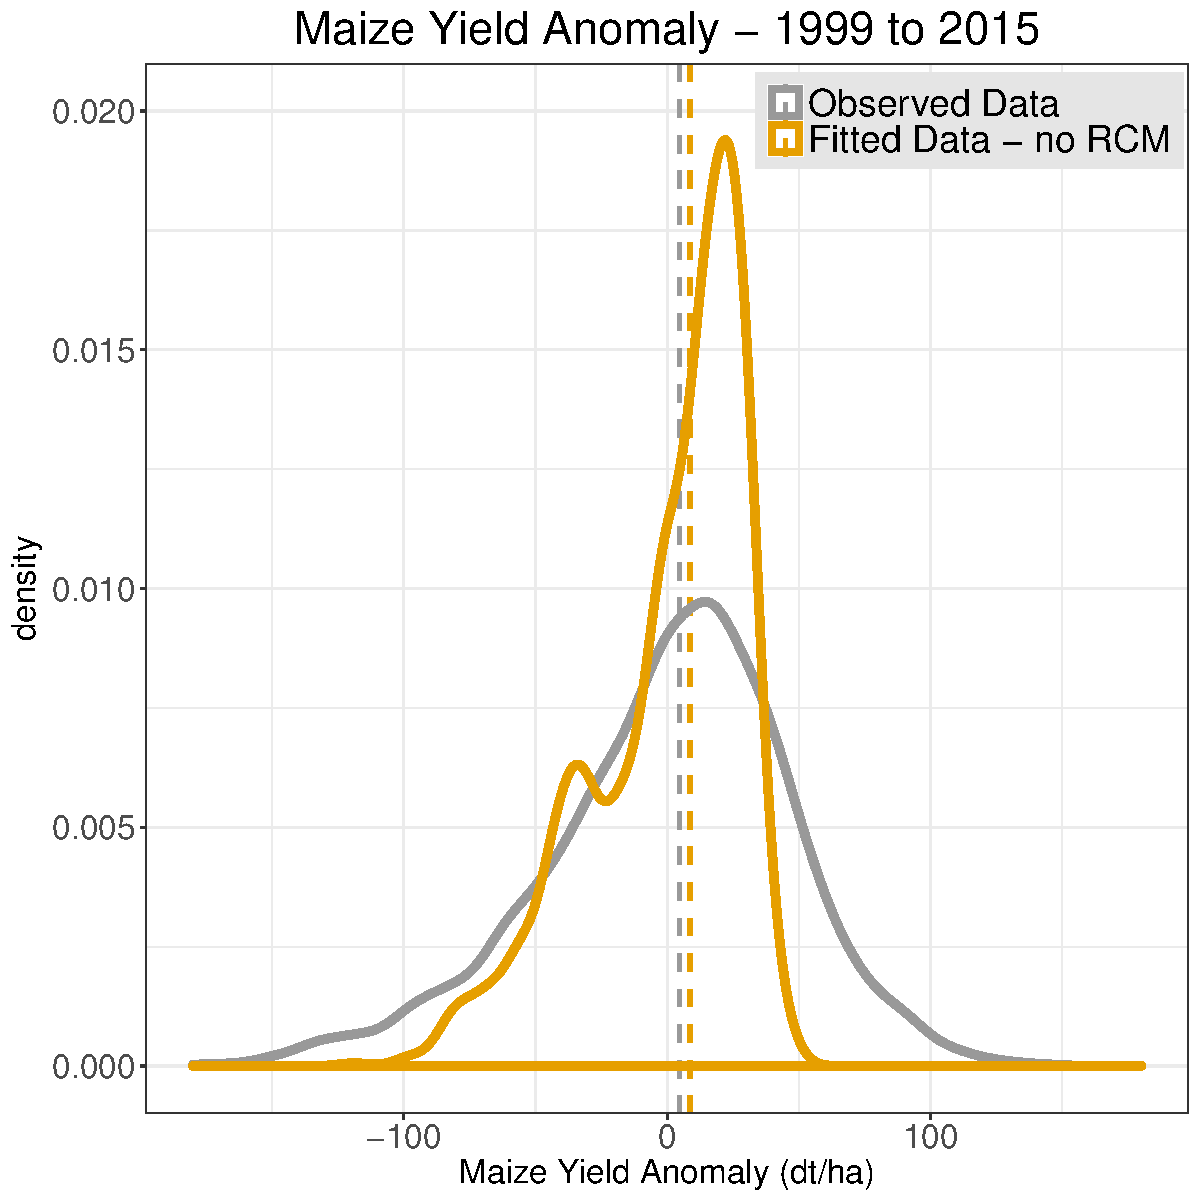
\includegraphics[width=1\textwidth]{figures/Density_1999-2015_Anomalies_sMA_lm_fit_SMI_6_Jun_Aug.pdf}
	\caption{Density Plot of the observed silage Maize Anomaly Data against the predicted data with the standard model considering SMI of June and August and
		Meteorology of July using observed data. The time period is 1999 to 2015.}
\end{figure}

%\begin{figure}
%	\label{density:1bf}
%	\centering
%	\includegraphics[width=1\textwidth]{figures/DensityPlots/Density_1999-2015_Anomalies_allModels.pdf}
%	\caption{Density Plot of the observed silage Maize Anomaly Data against the predicted data with the standard model considering all models using observed data. The time period is 1999 to 2015.}
%\end{figure}


%\begin{figure}
%	\label{scatter:2f}
%	\centering
%	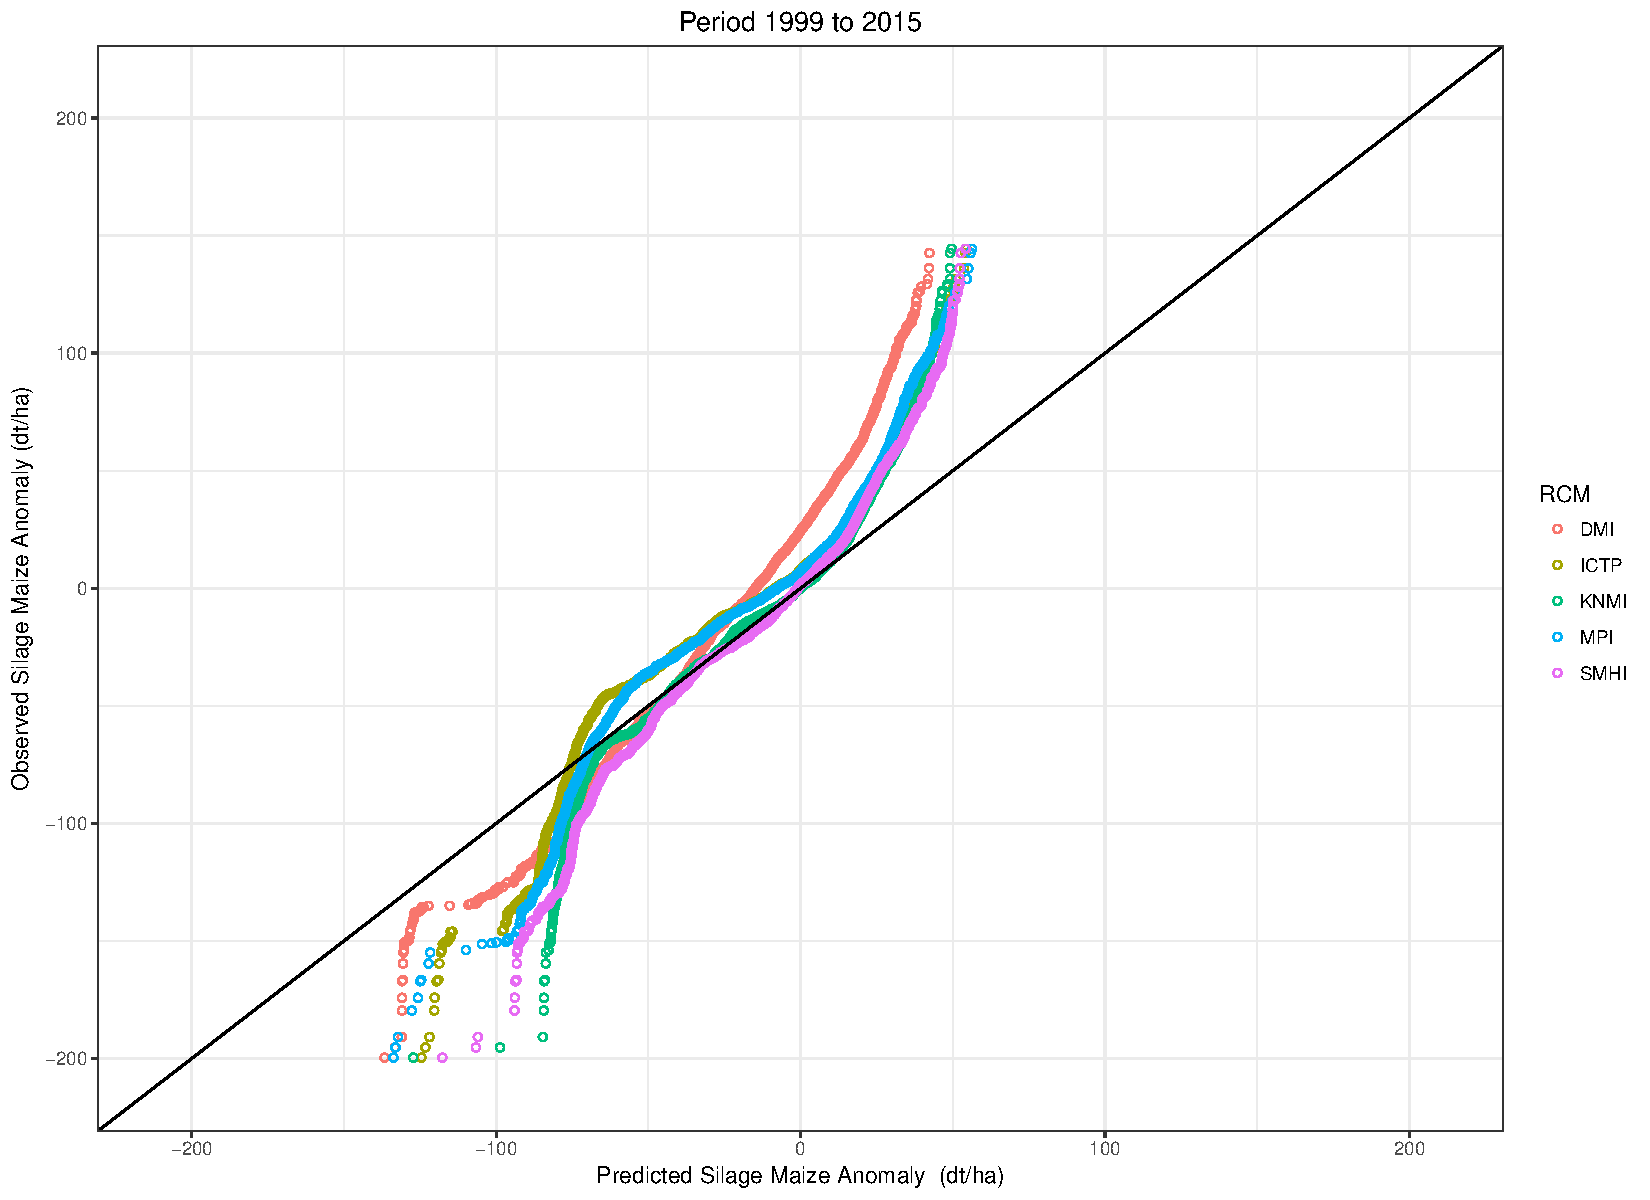
\includegraphics[width=1\textwidth]{figures/Scatterplots/Climate_1999-2015_RCMs.pdf}
%	\caption{Scatterplot of the observed silage Maize Anomaly Data against the predicted data with the standard model considering SMI of June and August and
%		Meteorology of July using data derived from the RCMs. The time period is 1999 to 2015.}
%\end{figure}

\begin{figure}
	\label{density:2f}
	\centering
	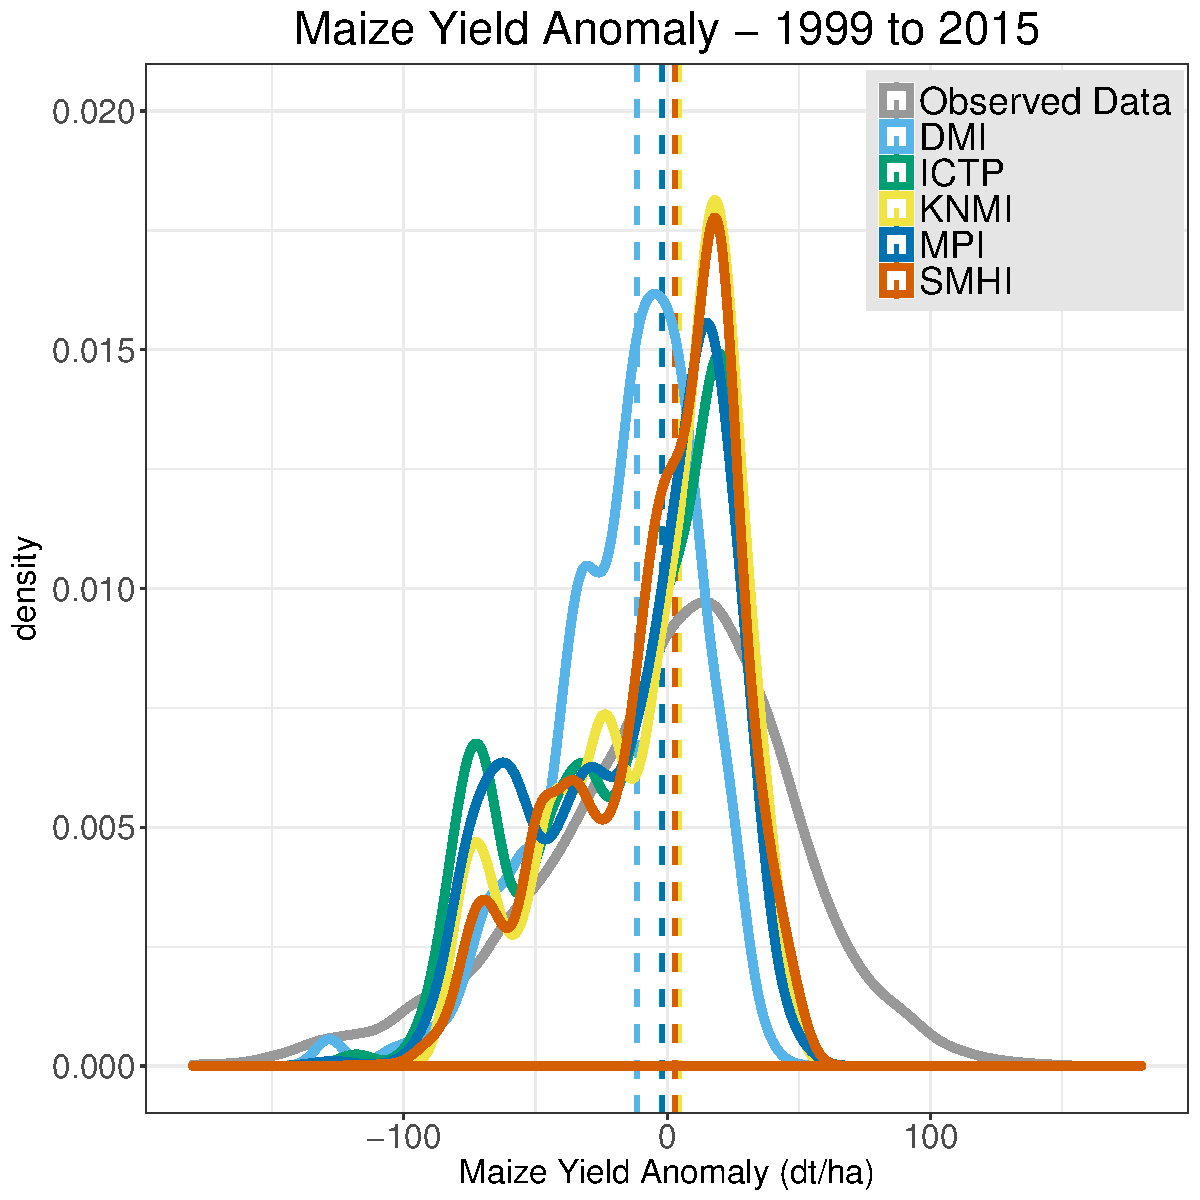
\includegraphics[width=1\textwidth]{figures/Density_Climate_1999-2015_RCMs.pdf}
	\caption{Density Plot of the observed silage Maize Anomaly Data against the predicted data with the standard model considering SMI of June and August and
		Meteorology of July using data derived from the RCMs. The time period is 1999 to 2015.}
\end{figure}


%\begin{figure}
%	\label{scatter:3af}
%	\centering
%	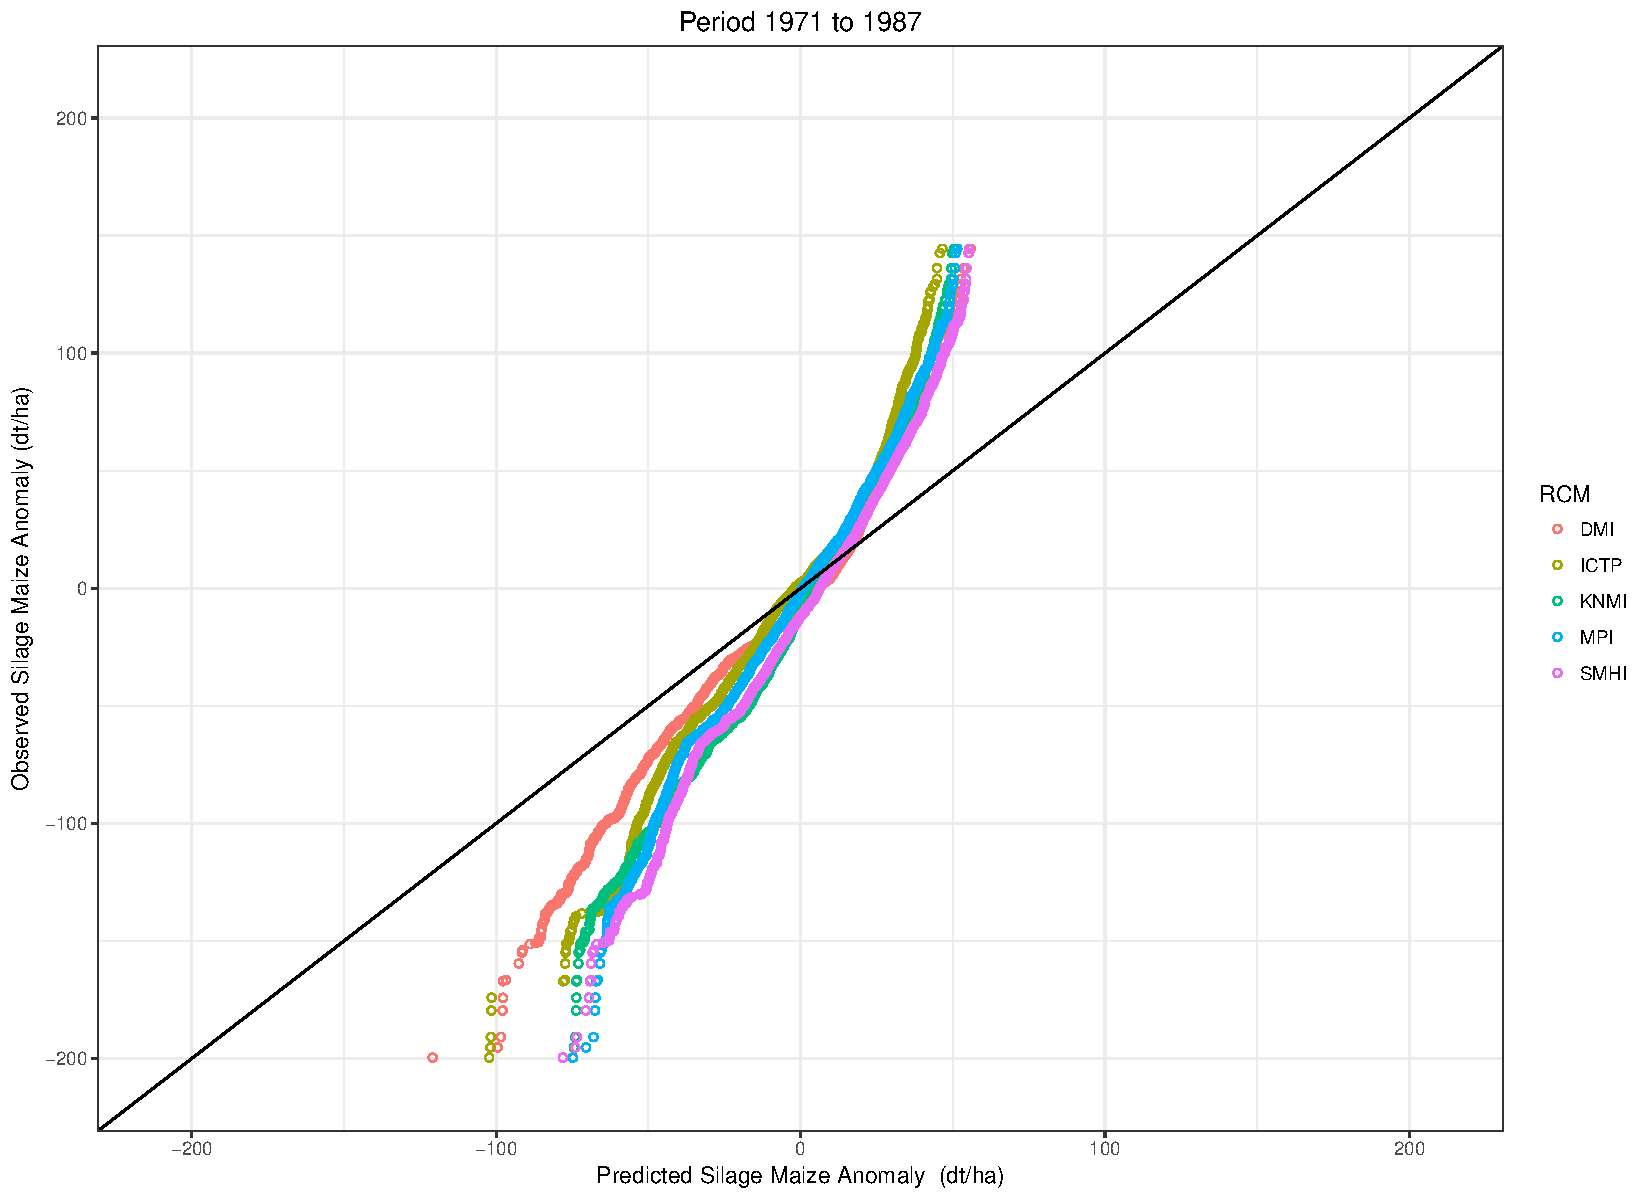
\includegraphics[width=1\textwidth]{figures/Scatterplots/Climate_1971-1987_RCMs.pdf}
%	\caption{Scatterplot of the observed silage Maize Anomaly Data against the predicted data with the standard model considering SMI of June and August and
%		Meteorology of July using data derived from the RCMs. The time period is 1997 to 1993. This is interesting since we use the time period of 1971 - 2000 as reference against which we compare the climate periods.}
%\end{figure}

%\begin{figure}
%	\label{scatter:3bf}
%	\centering
%	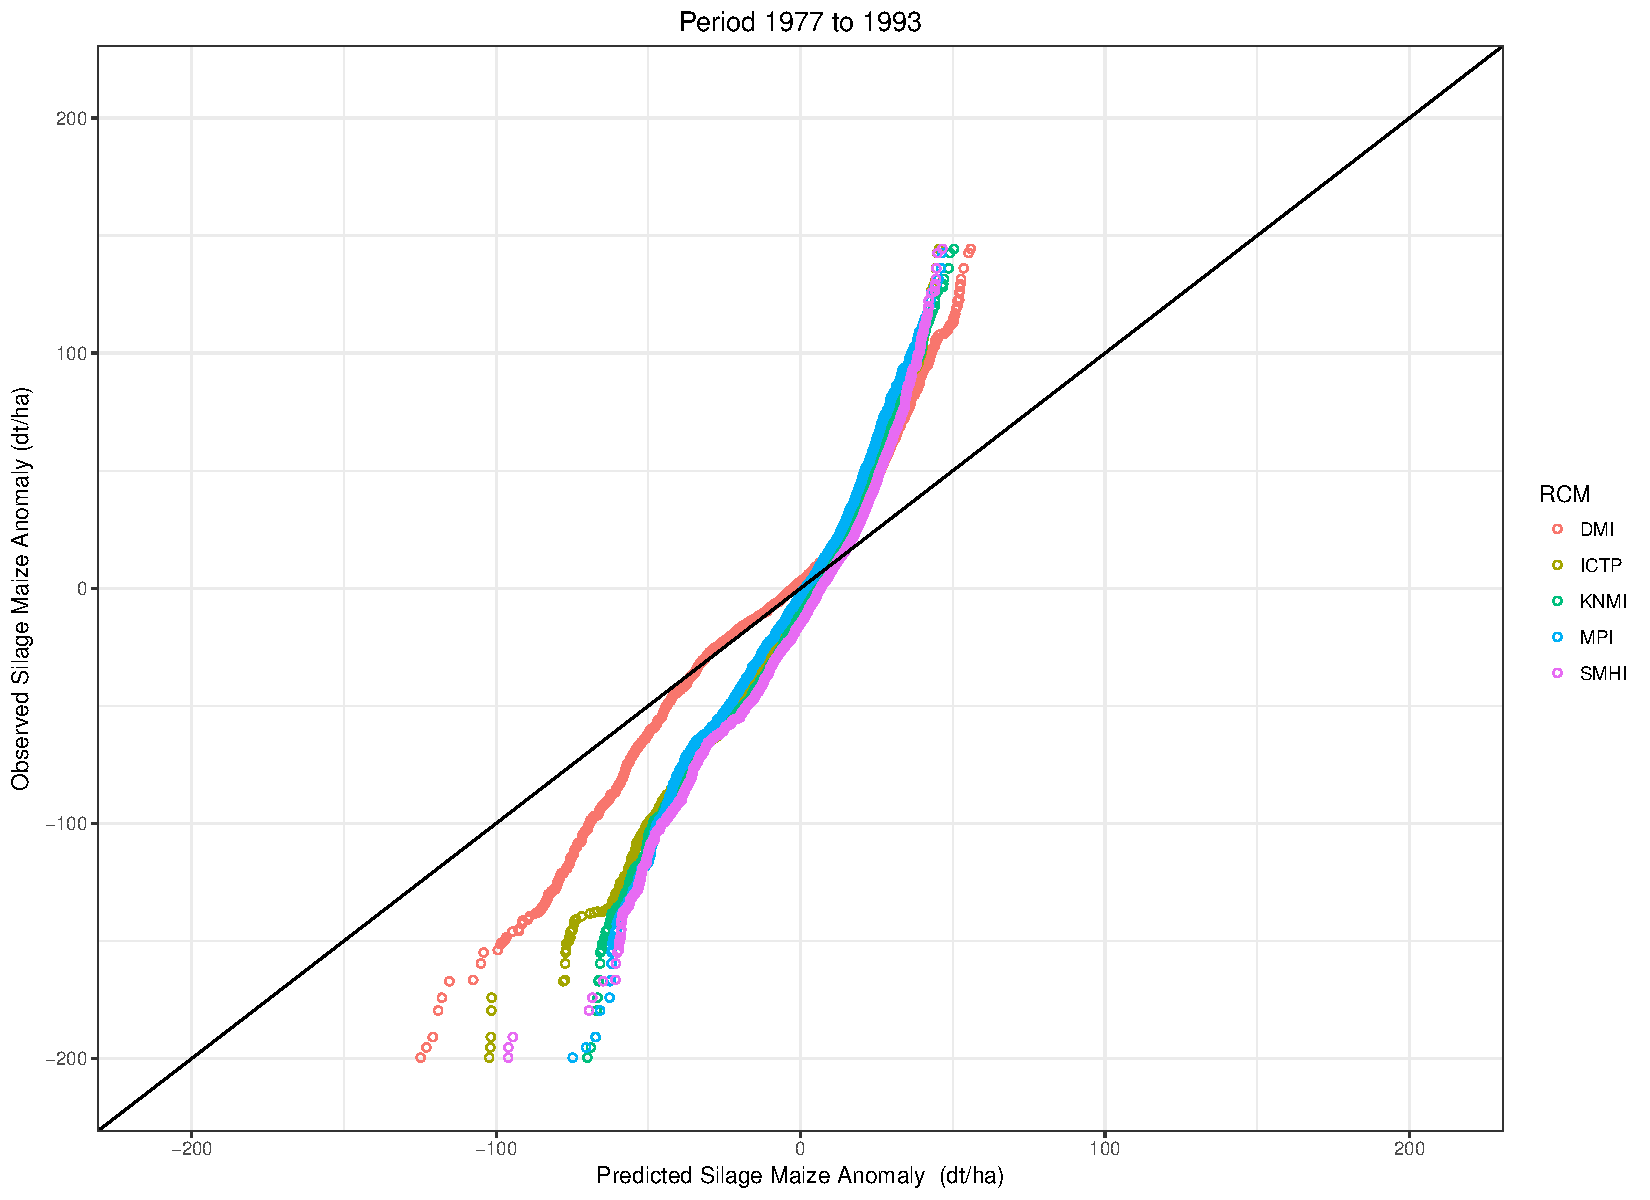
\includegraphics[width=1\textwidth]{figures/Scatterplots/Climate_1977-1993_RCMs.pdf}
%	\caption{Scatterplot of the observed silage Maize Anomaly Data against the predicted data with the standard model considering SMI of June and August and
%		Meteorology of July using data derived from the RCMs. The time period is 1977 to 1993. This is interesting since we use the time period of 1971 - 2000 as reference against which we compare the climate periods.}
%\end{figure}

%\begin{figure}
%	\label{scatter:3cf}
%	\centering
%	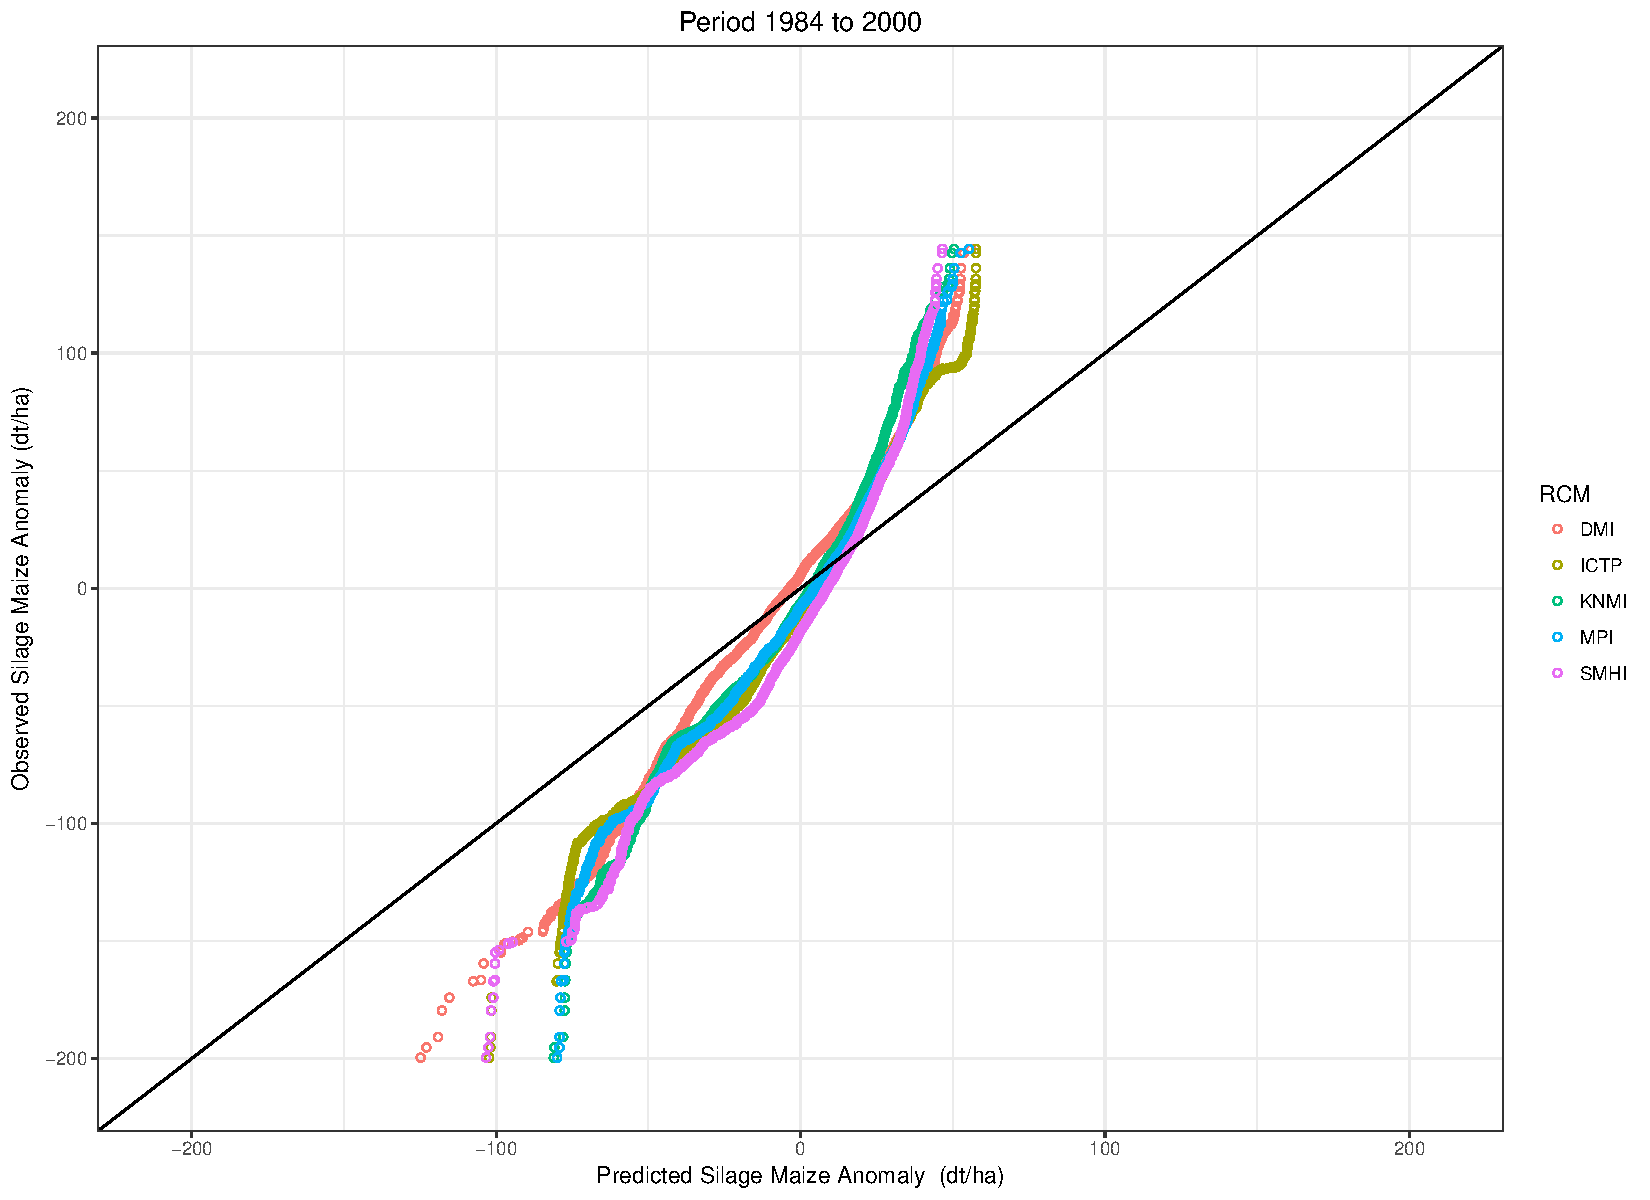
\includegraphics[width=1\textwidth]{figures/Scatterplots/Climate_1984-2000_RCMs.pdf}
%	\caption{Scatterplot of the observed silage Maize Anomaly Data against the predicted data with the standard model considering SMI of June and August and
%		Meteorology of July using data derived from the RCMs. The time period is 1984 to 2000. This is interesting since we use the time period of 1971 - 2000 as reference against which we compare the climate periods.}
%\end{figure}

%\begin{figure}
%	\label{density:3f}
%	\centering
%	\includegraphics[width=1\textwidth]{figures/DensityPlots/Density_Climate_1977-1993_RCMs.pdf}
%	\caption{Scatterplot of the observed silage Maize Anomaly Data against the predicted data with the standard model considering SMI of June and August and
%		Meteorology of July using data derived from the RCMs. The time period is 1977 to 1993. This is interesting since we use the time period of 1971 - 2000 as reference against which we compare the climate periods.}
%\end{figure}


\subsection{Projections}

\subsubsection{Violin Plots}
\begin{figure}
	\label{violin:1f}
	\centering
	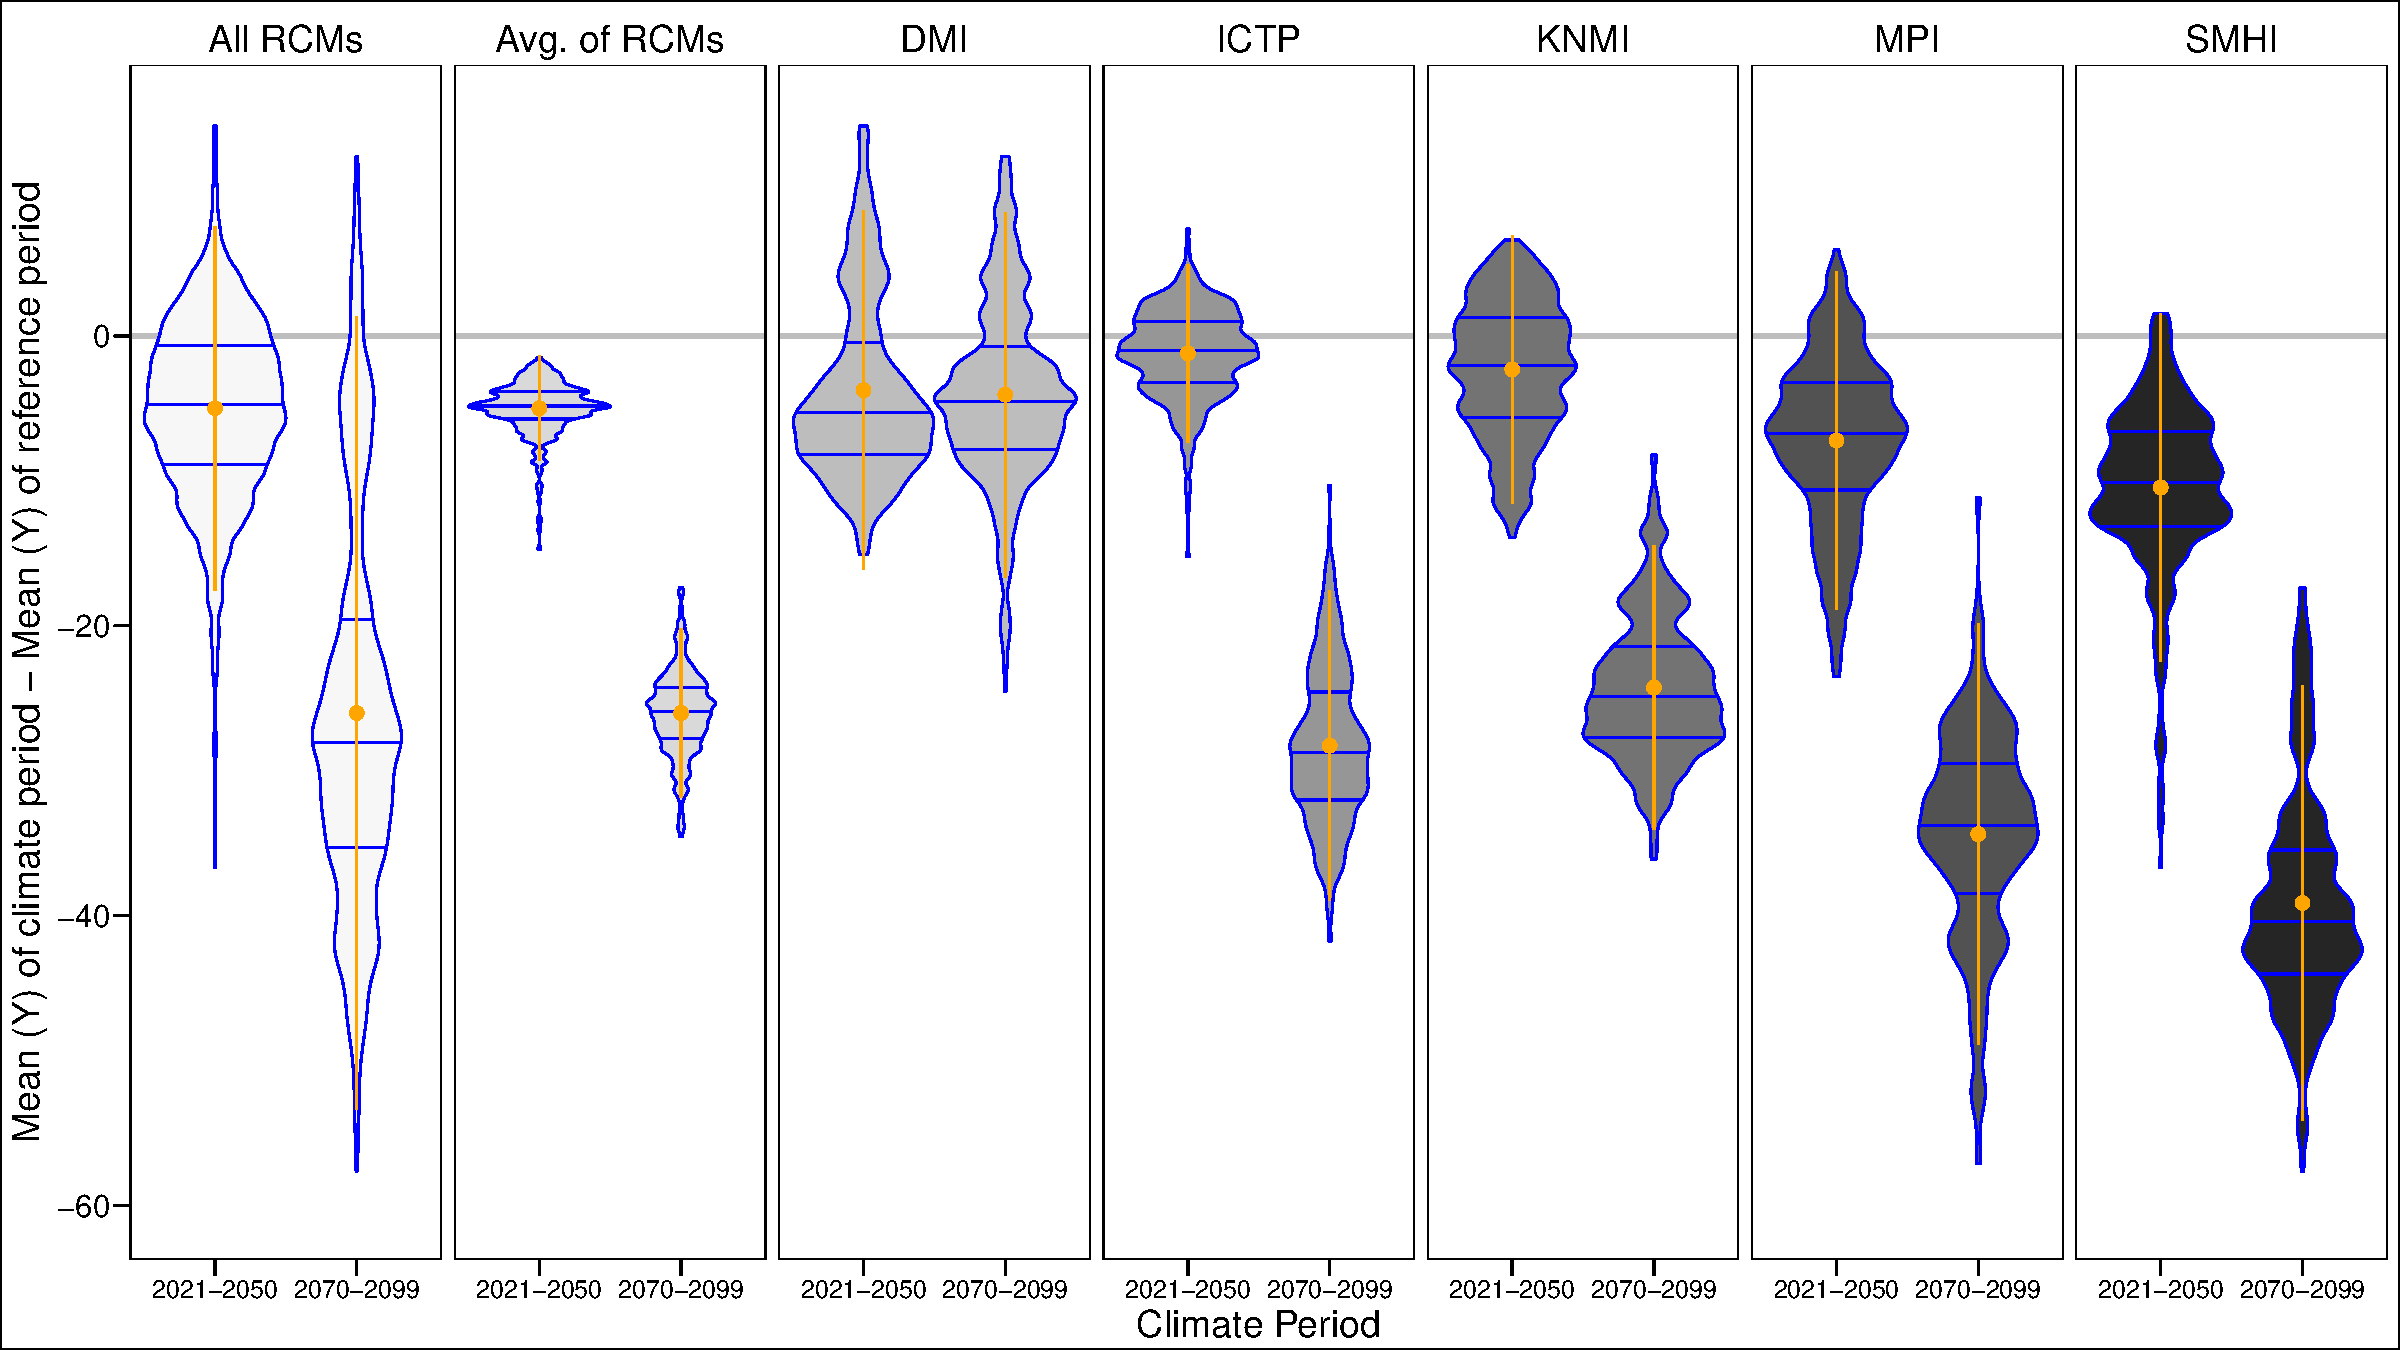
\includegraphics[width=1\textwidth]{figures/ViolinPlot_meanMinusMean.pdf}
	\caption{Violin Plot of the predicted yield for the periods 2021 - 2050 and 2070 - 2099 compared against the reference period 1971 - 2000. The first panel shows the cumulated results for all RCMs, the other five for each RCM separately.}
\end{figure}

\subsubsection{Maps of Results}
\begin{figure}
	\label{map:1f}
	\centering
	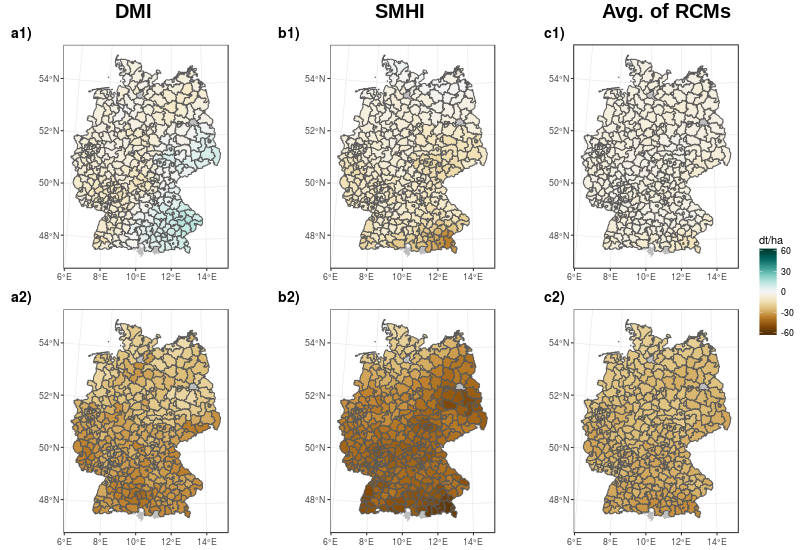
\includegraphics[width=1\textwidth]{figures/plot_mean_yield_SMI_6_Jun_Aug_ExtremesAndAvg.png}
	\caption{}
\end{figure}



\subsubsection{Maps of Structural Patterns of Yield and Explanatory Variables.}
\begin{figure}
	\label{map:1f}
	\centering
	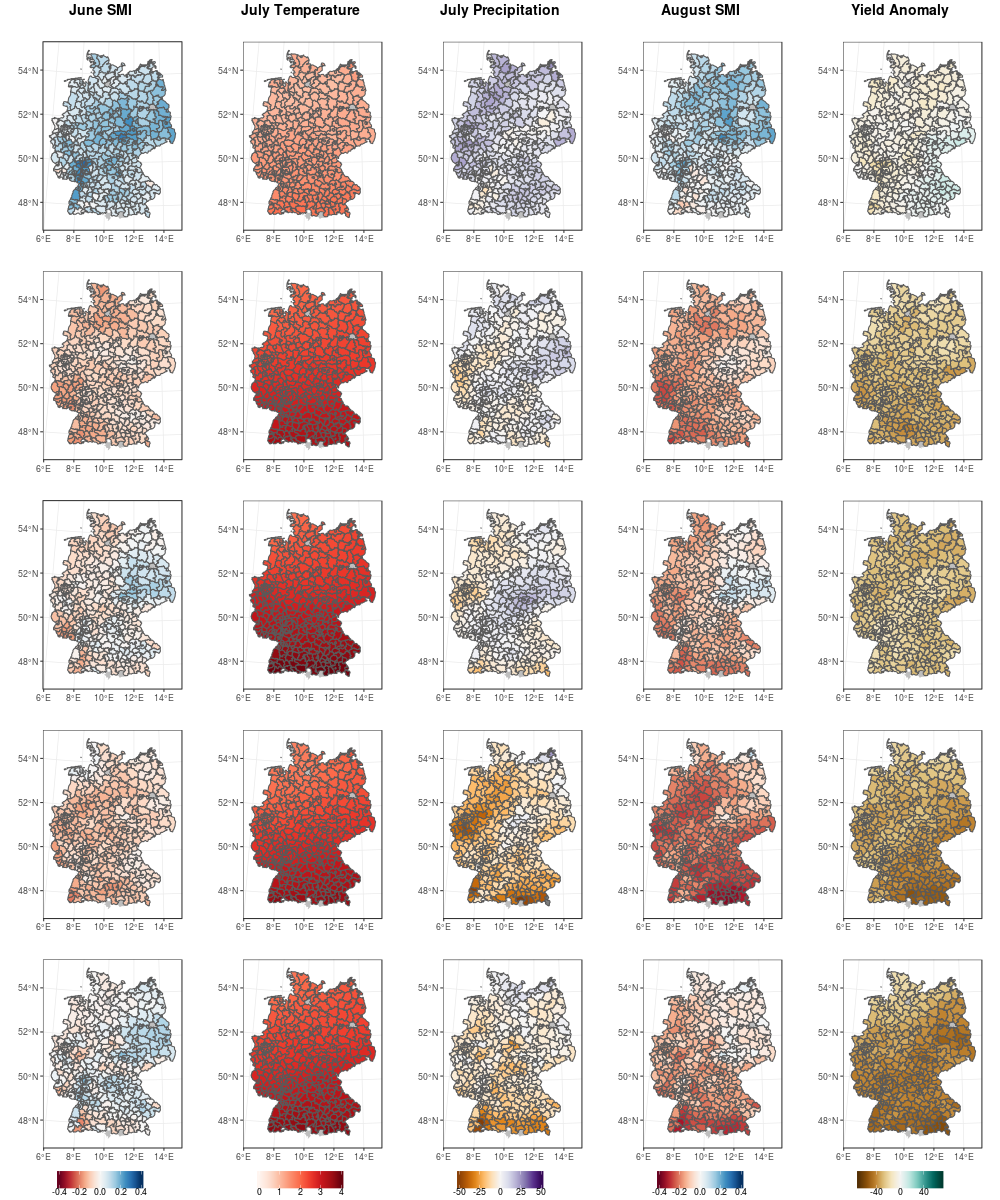
\includegraphics[width=1\textwidth]{figures/structural.png}
	\caption{}
\end{figure}







\section{Discussion}
% \ack
% \appendix 

% Wilcoxon 
\begin{figure}
	\label{map:2f}
	\centering
	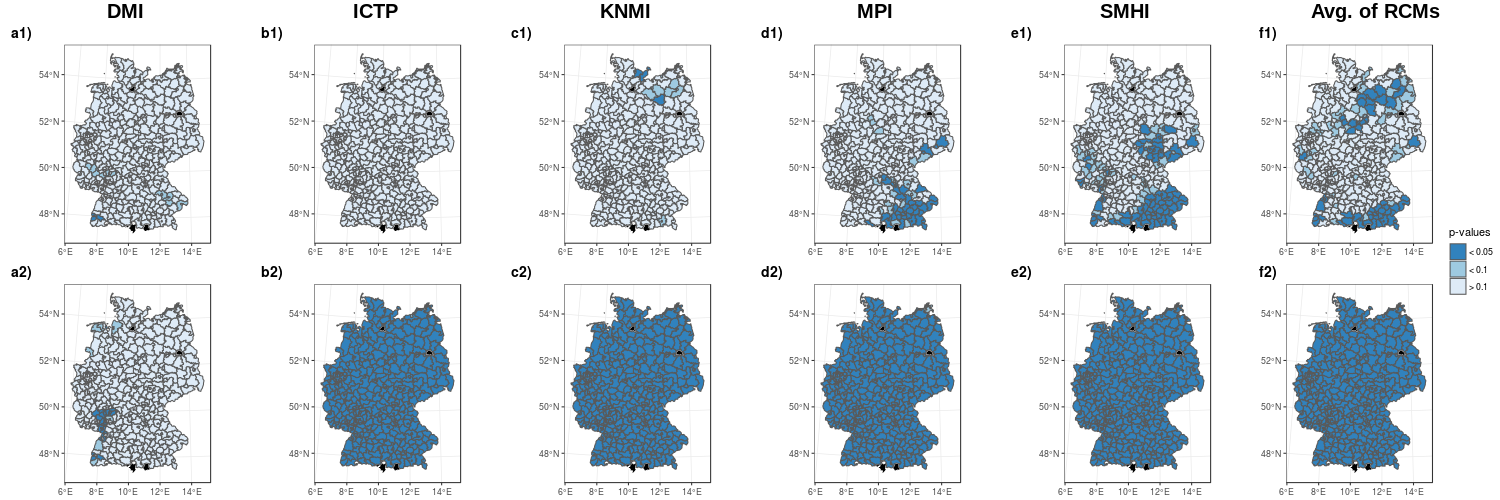
\includegraphics[width=1\textwidth]{figures/Wilcoxon_AllRCMs.png}
	\caption{}
\end{figure}


\newcommand{\newblock}{}
\bibliographystyle{dcu} %{dcu} 
\bibliography{Mendeley.bib}
%\bibliography{high_flows}

\end{document}



